\documentclass[Thesis.tex]{subfiles}
\begin{document}
\chapter{Simulation and results}

The \gls{ROS} package built for \gls{AMCL6D} also includes a simple tool to simulate a robot pose. This tool was used to simulate and test the algorithm. The algorithm can be visualized using RVIZ, which is illustrated in \figRef{fig:amclaction}.
The performance of the algorithm was tested on different maps and with different resolutions. To assure accuracy, for each map there was a random but arbitrary sequence of motions defined which was repeated for each trial. The simulated camera for the ray tracing always had aperture angles of $90^\circ$ (horizontal) and $60^\circ$ (vertical).

\begin{figure}
\centering
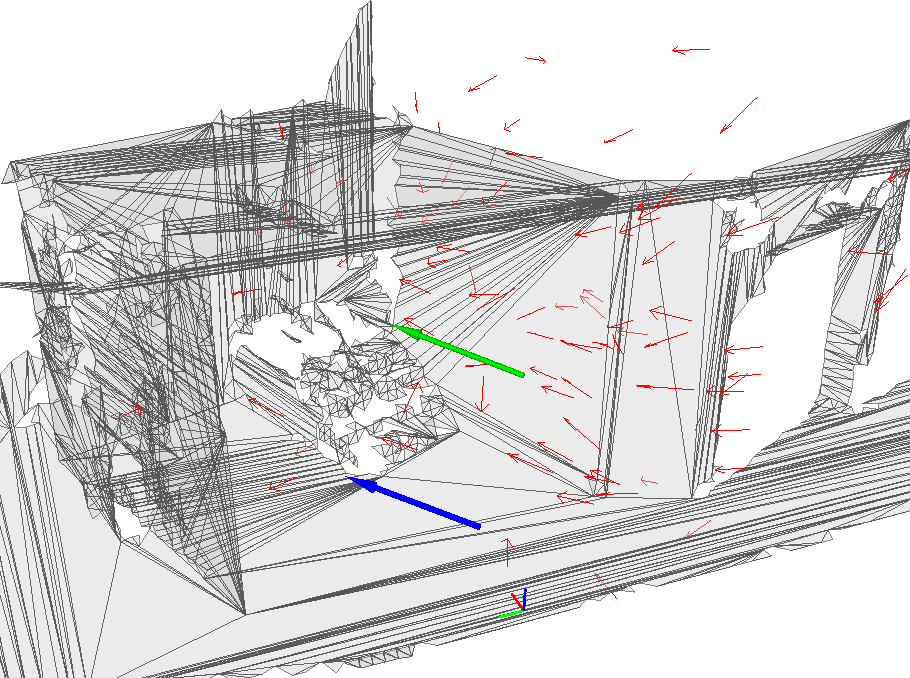
\includegraphics[width=.8\columnwidth]{pics/amclaction}
\caption[AMCL6D localization]{The localization of AMCL6D. The small red arrows illustrate the samples, the green arrow the likeliest sample and the blue arrow the real value.}
\label{fig:amclaction}
\end{figure}

\section{Performance in different maps}
The performance is measured by taking the distance between the simulated real pose and the best hypothesis after each time step, hence lower values mean better results. For the comparisons in these sections the euclidean distance between the poses' positions was used, as it has greater impact on the localization.


\begin{figure}\centering
\begin{tabularx}{\textwidth}{XlrrX}
  &\multicolumn{2}{c}{\small\bf Map and test properties} & \multirow{9}{*}{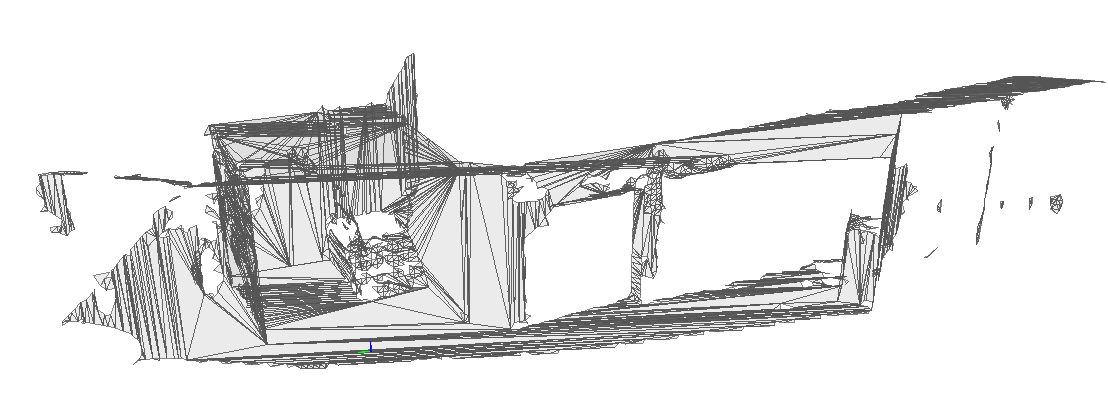
\includegraphics[width=.6\columnwidth]{pics/elvmap}}&\\
	&Vertex count & 3,774 &\\
  &Face count  & 3,924 &\\
  &Iterations  & 100 &\\
  &Resolution  & 65x45 &\\
  &Approx. Dimensions  & 6x23x4 &\\
  &&&\\
  &&&\\
  &&&\\
\end{tabularx}
\caption{Map and test properties: Elevator door}
\label{fig:elvmapprop}
\end{figure}

\begin{figure}\centering
\begin{tabularx}{\textwidth}{XlrrX}
  &\multicolumn{2}{c}{\small\bf Map and test properties} & \multirow{13}{*}{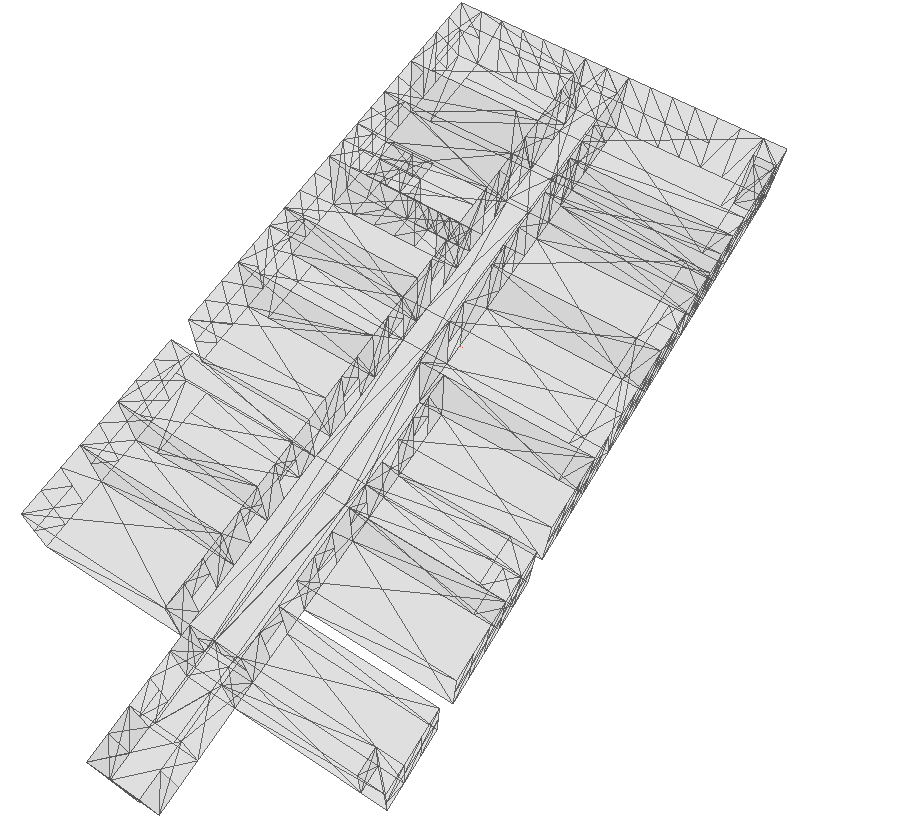
\includegraphics[width=.5\columnwidth]{pics/officemap}}&\\
	&Vertex count & 1,018 &\\
  &Face count  & 857 &\\
  &Iterations  & 100 &\\
  &Resolution  & 65x45 &\\
  &Approx. Dimensions  &15x33x8&\\
  &&&\\
  &&&\\
  &&&\\
  &&&\\
  &&&\\
  &&&\\
  &&&\\
\end{tabularx}
\caption{Map and test properties: Office corridor}
\label{fig:offmapprop}
\end{figure}

\subsection*{Elevator door}
The elevator door map is open on one side and has lots of holes. It is smaller in size than the office map, but has more vertices and faces.

The results in \figRef{fig:reselv} show that the algorithm is not capable of localizing the robot within 100 iterations. However it is interesting that the algorithm decreases the distance steadily during the first half of each experiment but after about 50 iterations it spikes far away and has problems to recover.

\subsection*{Office corridor}
The office corridor map is about seven times larger than the elevator door map, however it has less vertices and faces. This is due to its very regular structure. In contrast to the other map, the office corridor is complete and without any holes. 

The results illustrated in \figRef{fig:resoff} are worse than those of the elevator door map. In the office corridor the algorithm was not able to localize the robot, additionally the tendency observed in the first iterations in the elevator door map is not visible. This is most probably because the sample size of just 100 samples is really small and the map is huger than the other one. However for larger sample sizes the computational time of the ray tracer is not acceptable anymore, as it already was a huge bottleneck with different resolutions (see \secRef{sec:rtspeed}).

\begin{figure}
\centering
\begin{tikzpicture}
\begin{axis}[xlabel={Iterations}, ylabel={Distance},axis lines=left,width=.8\textwidth,height=.5\textwidth,legend entries={mean values},]
\addplot[thin, orange]        table [x=iter, y=avg, col sep=comma]  {data/elvavg.csv};
\draw[-,red] (axis cs:0,5.05) -- (axis cs:100,5.05);
\addplot[ultra thin, gray!90] table [x=iter, y=dist, col sep=comma] {data/elv3.txt};
\addplot[ultra thin, gray!80] table [x=iter, y=dist, col sep=comma] {data/elv4.txt};
\addplot[ultra thin, gray!70] table [x=iter, y=dist, col sep=comma] {data/elv5.txt};
\addplot[ultra thin, gray!60] table [x=iter, y=dist, col sep=comma] {data/elv6.txt};
\addplot[ultra thin, gray!50] table [x=iter, y=dist, col sep=comma] {data/elv7.txt};
\end{axis}
\end{tikzpicture}
\caption[Results elevator door map]{Trial results of the elevator door map. The red line shows the over all mean distance.}
\label{fig:reselv}
\end{figure}

\begin{figure}
\centering
\begin{tikzpicture}
\begin{axis}[xlabel={Iterations}, ylabel={Distance},axis lines=left,width=.8\textwidth,height=.5\textwidth,legend entries={mean values},legend style={at={(.2,1)},anchor=north west}]
\addplot[thin, orange]        table [x=iter, y=avg, col sep=comma]  {data/offavg.csv};
\draw[-,red] (axis cs:0,10.96) -- (axis cs:100,10.96);
\addplot[ultra thin, gray!90] table [x=iter, y=dist, col sep=comma] {data/off1.txt};
\addplot[ultra thin, gray!80] table [x=iter, y=dist, col sep=comma] {data/off2.txt};
\addplot[ultra thin, gray!70] table [x=iter, y=dist, col sep=comma] {data/off3.txt};
\addplot[ultra thin, gray!60] table [x=iter, y=dist, col sep=comma] {data/off4.txt};
\addplot[ultra thin, gray!50] table [x=iter, y=dist, col sep=comma] {data/off5.txt};
\end{axis}
\end{tikzpicture}
\caption[Results office corridor map]{Trial results of the office corridor map. The red line shows the over all mean distance.}
\label{fig:resoff}
\end{figure}

\clearpage
\section{Resolution of ray tracer}
To see how much impact the resolution of the sensor model has and if there are better resolutions, tests in the same elevator door map (\figRef{fig:elvmapprop}) with different resolutions of 100x80 (2 runs), 65x45 (5), 30x20 (5) were compared.

The mean results are illustrated in \figRef{fig:resresults}. As one can see, all resolutions perform similar and there is none which might be preferable over the others.

\begin{figure}
\centering
\begin{tikzpicture}
\begin{axis}[xlabel={Iterations}, ylabel={Distance},axis lines=left,width=.8\textwidth,height=.4\textwidth, legend style={at={(.5,1)},anchor=north}]
\addplot[red]    table [x=iter, y=avg, col sep=comma] {data/elvsavg.csv};
\addlegendentry{30x20}
\addplot[blue] table [x=iter, y=avg, col sep=comma] {data/elvavg.csv};
\addlegendentry{65x45}
\addplot[olive]  table [x=iter, y=avg, col sep=comma] {data/elvhavg.csv};
\addlegendentry{100x80}
\end{axis}
\end{tikzpicture}
\caption[Resolution trials]{Mean results of trials with different resolutions.}
\label{fig:resresults}
\end{figure}



\section{Ray tracing speed}\label{sec:rtspeed}
The algorithm performed very slow on the medium and high resolutions. While following the assumption that the ray tracer might be a bottleneck, the computation time of the ray tracer was tracked to find out its portion of time used during execution of the algorithm.
The results show that the ray tracer consumes most of the algorithm's running time, with rates varying between 93 and 96 percent. An improved ray tracer might therefor speed up the calculations enormously.
It can also be seen in \tableRef{tab:rtspeedrestable} that therefore smaller numbers of vertices and faces improve the time needed for the ray tracing. Using the mesh optimization software of the \gls{lvr} can thus lead to better results.

\begin{table}[h]
\begin{center}\footnotesize
\begin{tabular}{r|lc|rr|l}
\bf Run & \bf Map        & \bf Resolution & \bf Total time (s) & \bf RT time (s) & \bf \nicefrac{RT}{Total} (\%) \\ \toprule
1&Elevator&65x45&2139&2037&95.23\\
2&Elevator&65x45&2191&2085&95.16\\
3&Elevator&65x45&1867&1766&94.59\\
4&Elevator&65x45&2250&2146&95.38\\
5&Elevator&65x45&2084&1979&94.96\\
6&Elevator&65x45&2229&2124&95.29\\
7&Elevator&65x45&1944&1840&94.65\\
8&Elevator&30x20&481&457&95.01\\
9&Elevator&30x20&430&407&94.65\\
10&Elevator&30x20&528&504&95.45\\
11&Elevator&30x20&407&384&94.35\\
12&Elevator&30x20&464&443&95.47\\
13&Elevator&100x80&6166&5890&95.52\\
14&Elevator&100x80&6012&5730&95.31\\
15&Office&65x45&787&745&94.66\\
16&Office&65x45&764&722&94.50\\
17&Office&65x45&803&762&94.89\\
18&Office&65x45&786&737&93.77\\
19&Office&65x45&827&786&95.04\\
\bottomrule
\end{tabular}
\end{center}
\caption{Ray trace computation time comparisons}
\label{tab:rtspeedrestable}
\end{table}

\begin{figure}
\centering
\begin{tikzpicture}
	\begin{axis}[ymin=0,ymax=1,enlargelimits=0,xlabel={Different trials},ylabel={Ray tracing time / total time}, ybar interval = 0.4]
		\addplot[green!20!black,fill=green!50!white, name path=f] table[x=trial,y=per,col sep=comma] {data/rtres_100.csv}; 
		%\path[name path=ax] (axis cs:0,0) --(axis cs:19,0);
 		%\path[name path=ay] (axis cs:0,1) --(axis cs:19,1);
	\end{axis}
	\begin{axis}[ymin=0,ymax=1,enlargelimits=0,axis lines=none, ybar interval = 0.4]
  		\addplot[red!20!black,fill=red!50!white, name path=f] table[x=trial,y=per,col sep=comma] {data/rtres.csv};
 		%\path[name path=ax] (axis cs:0,0) --(axis cs:19,0);
 		%\path[name path=ay] (axis cs:0,1) --(axis cs:19,1);
 	\end{axis}
\end{tikzpicture}
\caption[Ray tracer computation time]{Comparison of the total time to ray trace time. The total execution time for each trial is set to 1. The red area is the time consumption by the ray tracer.}
\label{fig:rttimebenchmark}
\end{figure}

\section{Summary}
\gls{AMCL6D} initially performed well on a small map, independently from the ray tracer's resolution. However, once it got close to the real value it suddenly jumps far away. This makes it less useful in pose tracking than I initially hoped for. Additionally it was found that the ray tracer is really slow and throttles down the whole approach. Maybe replacing the ray tracer allows for more iterations in reasonable time frames and thus for a recovery from the loss of the pose tracking.




\end{document}
